\documentclass[12pt,a4paper]{extarticle}
\usepackage[utf8]{inputenc}
\usepackage[T5]{fontenc}
\usepackage{geometry}
\geometry{a4paper, left=1.5cm, right=1cm, top=1.5cm, bottom=1.5cm, headheight=20pt, headsep=15pt, footskip=28pt}
\usepackage{enumitem}
\usepackage{amssymb}
\usepackage{setspace}
\usepackage{tikz}
\definecolor{book}{RGB}{58,90,172}
\newcommand{\noteicon}{\textcolor{book}{$\blacktriangleright$}}
\usetikzlibrary{patterns, patterns.meta, calc} % Thêm patterns.meta vào đây
% Gọi package nằm trong thư mục con template
\usepackage{../template/mngocbox}

\begin{document}
\onehalfspacing

% Sử dụng ngoặc vuông [...] để thay đổi linh hoạt các thông số
\makeheadbox[headerright={Tổng ôn 10-11},chude={CHỦ ĐỀ 04},tieude={Oxy, ba đường conic},dinhdang={Hình học},lop={12 },gv={Nguyễn Lê Minh Ngọc}]

\vspace{2em}
\makeheading{IV}{Đề kiểm tra}
\textbf{Câu 14.} Một vận động ném đĩa đã vung đĩa theo một đường tròn $(C)$ có phương trình là $(x - 1)^2 + (y - 1)^2 = \dfrac{169}{144}$. Khi đó, người đó vung đĩa đến vị trí điểm $M\left(\dfrac{17}{12}; 2\right)$ thì buông đĩa. Viết phương trình tiếp tuyến của đường tròn $(C)$ tại điểm $M$.
\begin{center}
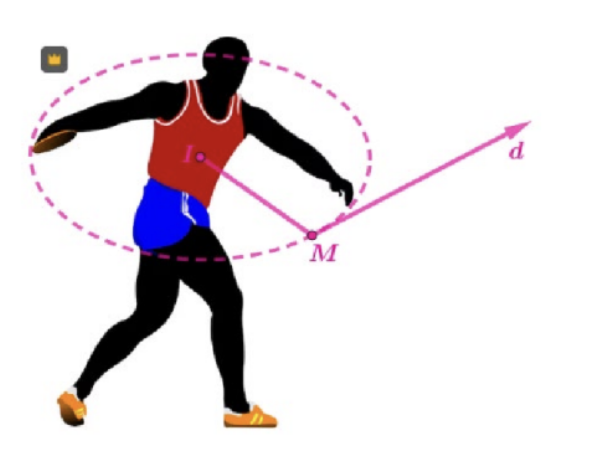
\includegraphics[width=0.3\textwidth]{5.14.png}
\end{center}
$\Rightarrow$ Đáp số: ..........

\textbf{Câu 15.} Tọa độ trong hệ thống kiểm soát phòng không trong không quân Việt Nam của một hệ thống rađa trong phạm vi bán kính $10$ km trở lại. Nếu một vật thể lạ di chuyển qua hệ thống trên không lý do sẽ có nguy cơ bị bắn hạ để bảo vệ an toàn trên vùng trời. Chọn hệ quy chiếu điểm ngắm là gốc tọa độ $O$. Hỏi máy bay đang bay ở tọa độ $M(6; 7)$ trên bầu trời có bị lọt vào tầm ngắm không? Vì sao?
\begin{center}
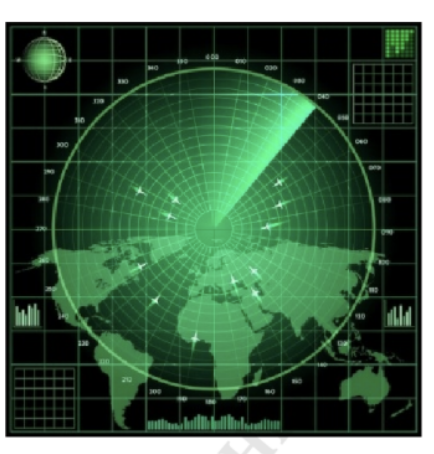
\includegraphics[width=0.3\textwidth]{5.15.png}
\end{center}
$\Rightarrow$ Đáp số: ..........
\textbf{Câu 9.} Để trang trí cho một lễ hội đầu xuân, từ một mảnh vườn hình elip có chiều dài trục lớn là $10$ m, chiều dài trục nhỏ là $4$ m. Ban tổ chức vẽ một đường tròn có đường kính bằng độ dài trục nhỏ và có tâm trùng với tâm của elip như hình vẽ. Biết diện tích hình elip có độ dài trục lớn, trục bé lần lượt là $a, b$ được tính theo công thức $S = \pi ab$.

Trên hình tròn người ta trồng hoa với giá $100\,000 \text{ đồng/m}^2$, phần còn lại của mảnh vườn người ta trồng cỏ với giá $60\,000 \text{ đồng/m}^2$ (biết giá trồng hoa và trồng cỏ bao gồm cả công và cây). Hỏi ban tổ chức cần bao nhiêu tiền để trồng hoa và cỏ (số tiền làm tròn đến hàng nghìn).
\begin{center}
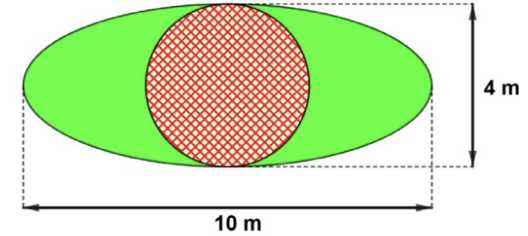
\includegraphics[width=0.5\textwidth]{6.9.png}
\end{center}
$\Rightarrow$ Đáp số: ..........

\textbf{Câu 10.} Dọc theo bờ biển, người ta thiết lập hệ thống định vị vô tuyến dẫn đường tầm xa để truyền tín hiệu cho máy bay hoặc tàu thuỷ hoạt động trên biển. Trong hệ thống đó có hai đài vô tuyến đặt lần lượt tại địa điểm $A$ và địa điểm $B$, khoảng cách $AB = 650$ km. Giả sử có một con tàu chuyển động trên biển với quỹ đạo là hypebol nhận $A$ và $B$ là hai tiêu điểm.

Khi đang ở vị trí $P$, máy thu tín hiệu trên con tàu chuyển đổi chênh lệch thời gian nhận các tín hiệu từ $A$ và $B$ thành hiệu khoảng cách $|PA - PB|$. Giả sử thời gian con tàu nhận được tín hiệu từ $B$ trước khi nhận được tín hiệu từ $A$ là $0,0012$ s. Vận tốc di chuyển của tín hiệu là $3.10^5$ m/s.
\begin{center}
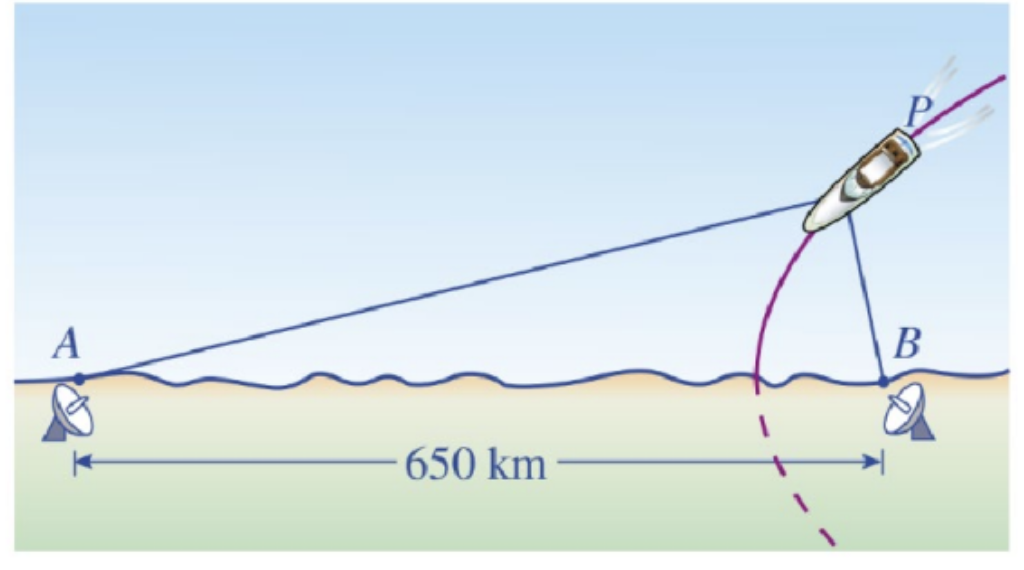
\includegraphics[width=0.5\textwidth]{6.10.png}
\end{center}
a) Lập phương trình hypebol mô tả quỹ đạo chuyển động của con tàu.

b) Chứng tỏ rằng tại mọi thời điểm trên quỹ đạo chuyển động thì thời gian con tàu nhận được tín hiệu từ $B$ trước khi nhận được tín hiệu từ $A$ luôn là $0,0012$ s.

\textbf{Câu 11.} Hình vẽ bên dưới mô phỏng mặt cắt ngang của một chiếc đèn có dạng parabol trong mặt phẳng tọa độ $Oxy$ ($x$ và $y$ tính bằng xăng-ti-mét). Hình parabol có chiều rộng giữa hai mép vành là $AB = 40$ cm và chiều sâu $h = 30$ cm ($h$ bằng khoảng cách từ $O$ đến $AB$). Bóng đèn nằm ở tiêu điểm $S$. Tham số tiêu của parabol bằng bao nhiêu?
\begin{center}
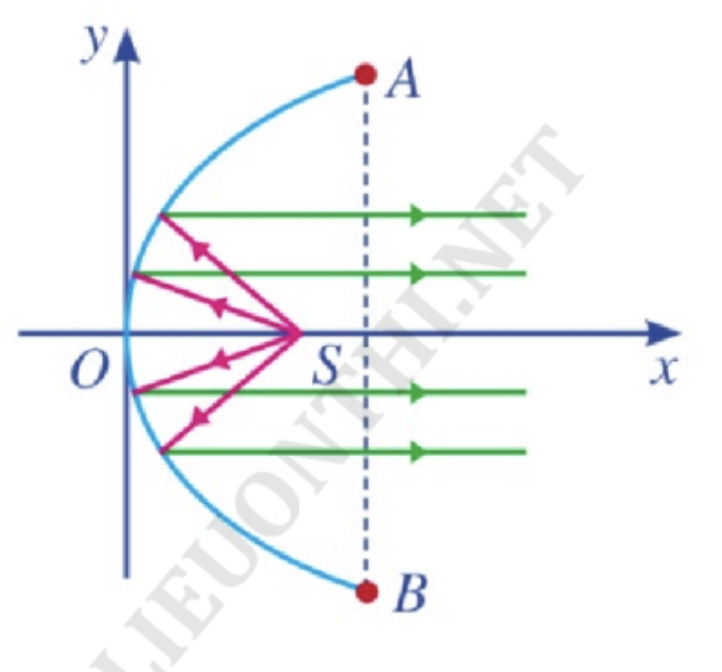
\includegraphics[width=0.5\textwidth]{6.11.png}
\end{center}
$\Rightarrow$ Đáp số: ..........
\end{document}